\subsection{供試体}
本実験では2種類の供試体を使用した。
液体酸素はインジェクタを通して供試体に流入する。燃料のあるプリバーナ部で燃焼をさせ、バッフルプレートを通して混合室部に流入しノズルから気体酸素と燃焼ガスが排出される。ノズルより下流は大気圧となっている。気化器の概略図を図\ref{fig:PBOut}に示す。
インジェクタには$\phi$0.3mmの孔が20個ある。それぞれの位置は軸中心から$\phi$12mmの位置に位相45°で8孔、$\phi$24mmの位置に位相30°で12孔とした。インジェクタ外観を図\ref{fig:Injector}に示す。
プリバーナ部の燃料の長さに応じてスペーサ(グラファイト)を詰めた。
供試体1は気化器内部の状態を可視化するために、プリバーナ部と混合室部の外殻にアクリル樹脂、混合室部の内壁に石英ガラスを使用した。
供試体2は基礎データ取得のために、プリバーナ部と混合室部の外殻にステンレスと混合室部の内壁にグラファイトを使用した。
プリバーナ部と混合室部を分けるバッフルプレートは$\phi$18mmの位置に孔を8孔開けた布ベークライト製のものと穴を4孔開けたグラファイト製のもの2種類を製作した。それぞれ穴の位相は45°と90°である。バッフルプレート外観を図\ref{Baffle}に示す。
ノズルは$\phi8.5mm$、グラファイトで製作した。
気化器1断面図を図\ref{fig:Chamber1},気化器2断面図を図\ref{fig:Chamber2}に示す。



\begin{figure}
\centering
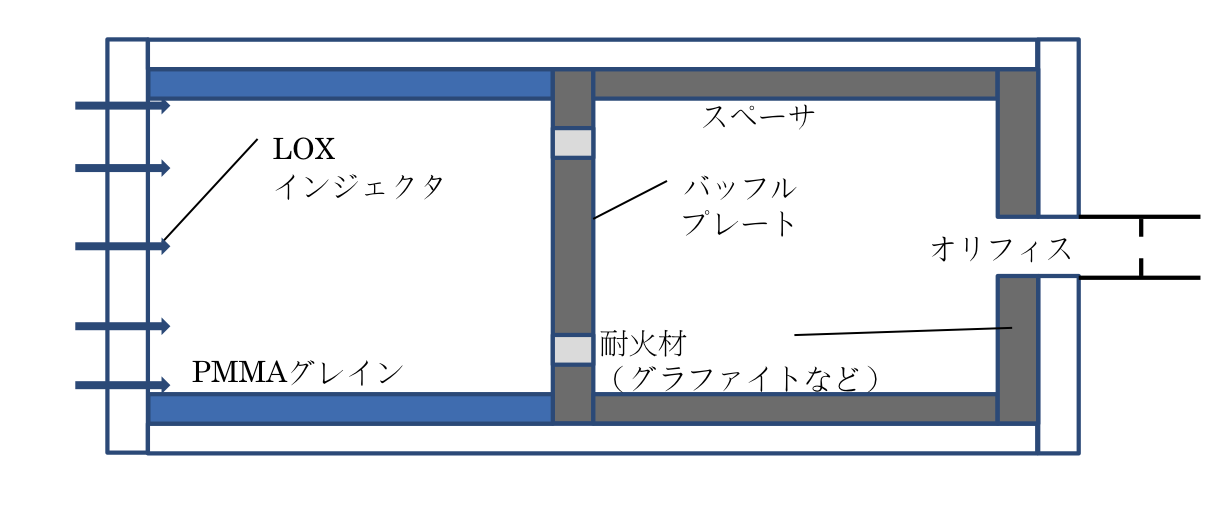
\includegraphics[width=15cm]{\FigAddTwo/PBImage.png}
\caption{プリバーナ概略図}
\label{fig:PBOut}
\end{figure}

\begin{figure}[htbp]
\begin{tabular}{cc}
\begin{minipage}{.5\textwidth}
\begin{center}
\centering
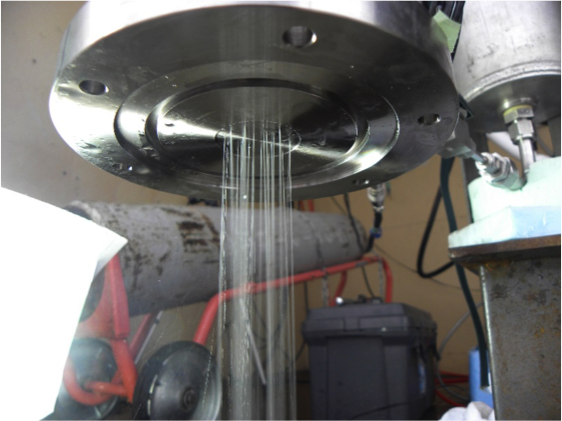
\includegraphics[width=7cm]{\FigAddTwo/Injector.png}
\caption{インジェクタ外観}
\label{fig:Injector}
\end{center}
\end{minipage}
\begin{minipage}{.5\textwidth}
\begin{center}
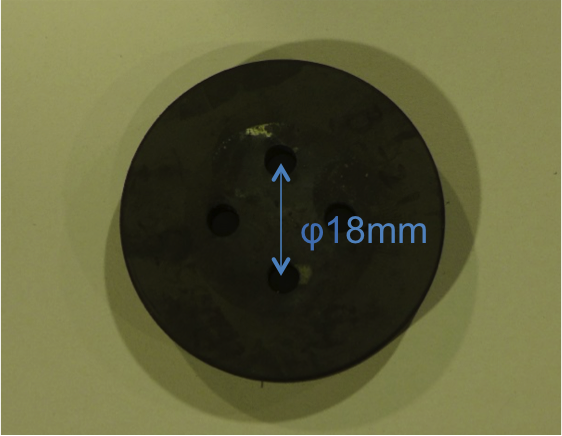
\includegraphics[width=7cm]{\FigAddTwo/BafflePlate.png}
\caption{バッフルプレート外観}
\label{fig:Baffle}
\end{center}
\end{minipage}
\end{tabular}
\end{figure}

\begin{figure}[htbp]
\begin{tabular}{cc}
\begin{minipage}{.5\textwidth}
\begin{center}
\centering
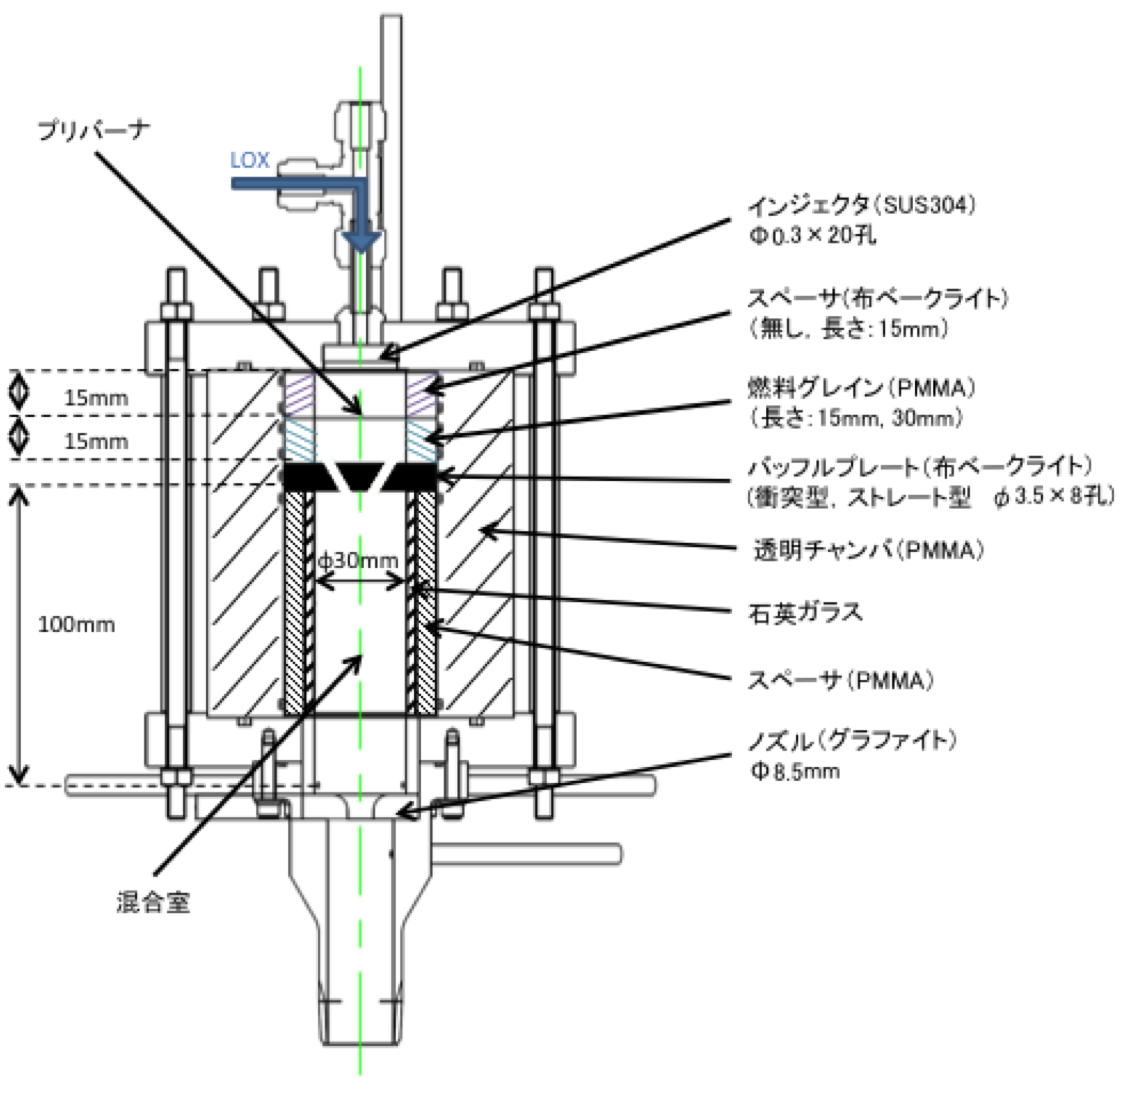
\includegraphics[width=7cm]{\FigAddTwo/Chamber1.jpg}
\caption{供試体1概要}
\label{fig:Chamber1}
\end{center}
\end{minipage}
\begin{minipage}{.5\textwidth}
\begin{center}
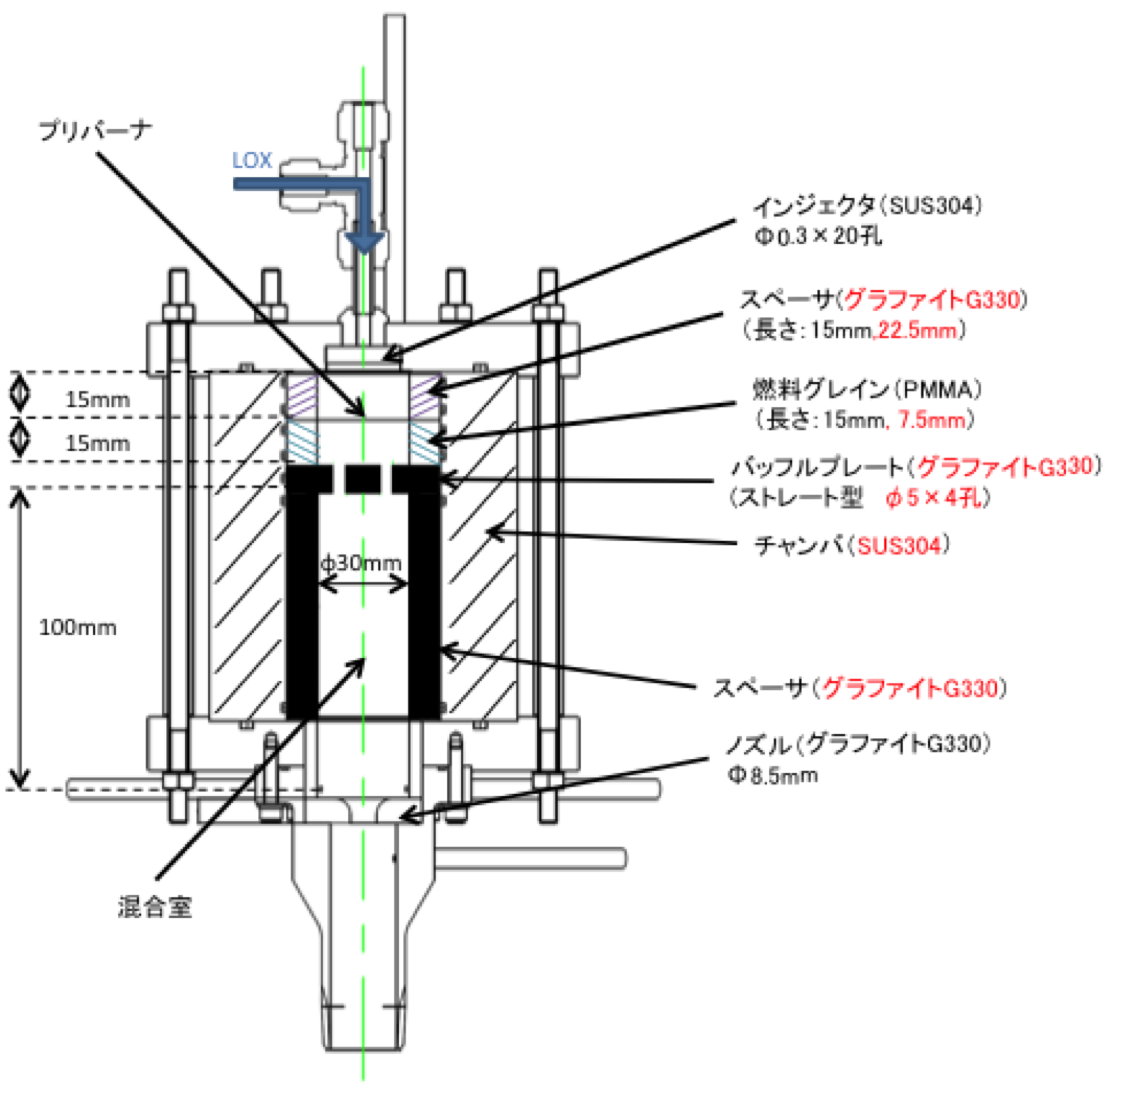
\includegraphics[width=7cm]{\FigAddTwo/Chamber2.jpg}
\caption{供試体2概要}
\label{fig:Chamber2}
\end{center}
\end{minipage}
\end{tabular}
\end{figure}

